% CVPR 2026 style paper for the course final assignment.
\documentclass[10pt,twocolumn,letterpaper]{article}

\usepackage[pagenumbers]{cvpr}
\usepackage{graphicx}
\usepackage{amsmath,amssymb}
\usepackage{booktabs}
\usepackage{array}
\usepackage{enumitem}
\usepackage{microtype}
\usepackage{balance}
\usepackage{tikz}
\usetikzlibrary{arrows.meta,positioning}

\setlength{\textfloatsep}{8pt plus 2pt minus 2pt}
\setlength{\floatsep}{8pt plus 2pt minus 2pt}
\setlength{\intextsep}{8pt plus 2pt minus 2pt}
\newcolumntype{L}[1]{>{\raggedright\arraybackslash}p{#1}}

\definecolor{cvprblue}{rgb}{0.21,0.49,0.74}
\usepackage[breaklinks,colorlinks,allcolors=cvprblue]{hyperref}

\newcommand{\system}{MicroMani}
\newcommand{\um}{\ensuremath{\mu\mathrm{m}}}

\title{Multimodal Teleoperation Data Collection and Alignment\\for Microdevice Assembly}

\author{Chun Xie\\
Student ID: 20255258070\\
School of Future Science and Engineering\\
Soochow University, Suzhou, China}

\begin{document}
\maketitle

\begin{abstract}
Microdevice assembly requires closed-loop operation at a scale where
micrometer-level motion, weak contact forces, visual occlusion, and
operator intent are tightly coupled. This paper presents an English
CVPR-style system design for \system, a multimodal teleoperation data
collection platform for microdevice assembly. The platform uses a
dual-arm six-degree-of-freedom micro-motion workstation, two Omega.7
haptic masters, global and wrist cameras, six-axis force/torque sensing,
and parallel grippers. The software stack connects a native hardware
abstraction layer, a backend recorder, asynchronous device buffers, and
a standardized episode format for robot learning. The key contribution
is not a new policy model, but a task-oriented data pipeline: each frame
records what the operator saw, what the operator commanded, where the
micro-motion stages moved, and what contact signal was measured. The
paper further relates the platform to microassembly, haptic
teleoperation, visual servoing, bimanual demonstration learning, and
large-scale robot dataset formats. A timestamp-based alignment method is
specified for synchronizing low-rate image streams with higher-rate
force, master-hand, gripper, and encoder signals.
\end{abstract}

\section{Introduction}
Microassembly is not ordinary assembly reduced in size. When components
shrink to the micro/nano scale, surface forces, adhesion, electrostatic
effects, viscous drag, and optical limits become central design
constraints. Classical microassembly surveys emphasize that
pick-and-place operations must be redesigned once surface forces dominate
gravity and inertia~\cite{cohn1998microassembly}. Haptic teleoperation
has also been studied as a way to make micromanipulation more intuitive,
because a human operator can remain in the loop while the remote tool
executes scaled motions and returns force cues~\cite{bolopion2013haptic}.

The present work focuses on a specific consequence of this scaling
problem: expert demonstrations for microdevice assembly are difficult to
collect in a reusable form. A useful learning episode must contain
multi-view images, micro-motion stage positions, haptic-master commands,
gripper states, and contact forces. If these modalities are not aligned,
the dataset may describe an incorrect causal relationship between
observation, action, and contact. This is especially harmful for modern
imitation-learning methods such as Action Chunking with Transformers
(ACT)~\cite{zhao2023aloha}, Diffusion Policy~\cite{chi2023diffusion},
and large robot datasets such as Open X-Embodiment~\cite{oneill2024openx}.

This paper turns the current \system\ engineering prototype into a
coherent CVPR-format system description. The goal is to specify how a
microdevice assembly workstation can collect demonstrations in a form
suitable for downstream robot learning. The system combines a
micro-motion mechanical layout, haptic teleoperation, visual observation,
six-axis force sensing, and timestamp-based dataset assembly. It follows
the practical direction of recent robot-learning infrastructure such as
LeRobot, which stresses standardized videos, state/action tables, and
reusable tools for real-world robot data~\cite{cadene2026lerobot}.

\begin{figure*}[t]
  \centering
  \begin{minipage}[t]{0.55\textwidth}
    \vspace{0pt}
    \centering
    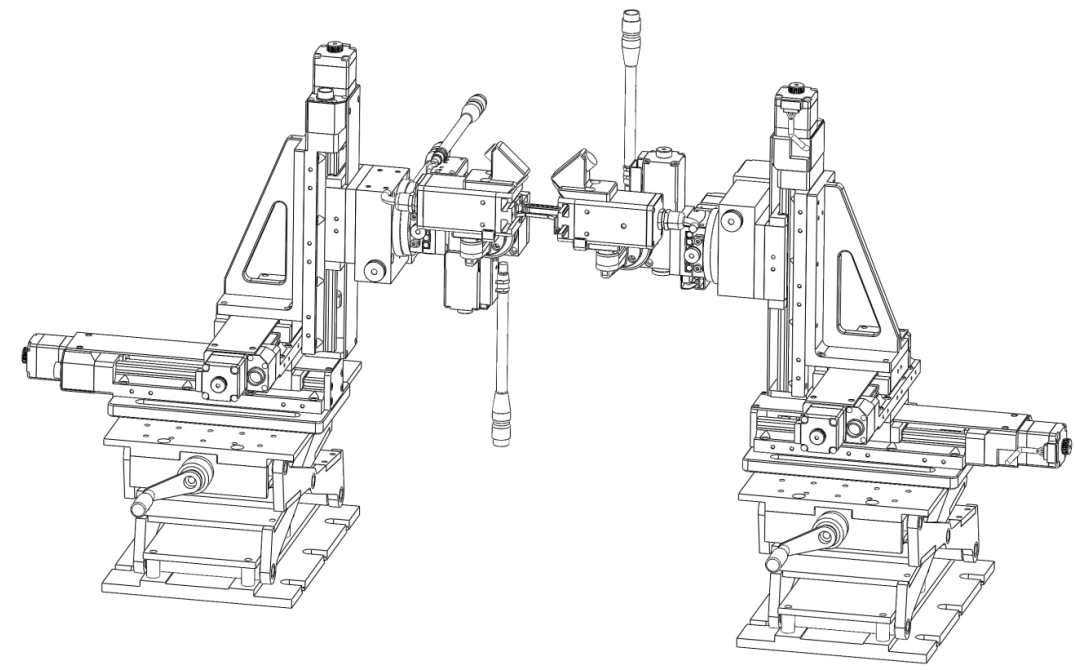
\includegraphics[width=0.98\linewidth]{figures/patent_overall_platform.png}
    \vspace{0.5mm}
    {\small (a) Dual-arm microdevice assembly workstation used as the physical layout.}
  \end{minipage}
  \hfill
  \begin{minipage}[t]{0.42\textwidth}
    \vspace{0pt}
    \centering
    \resizebox{0.98\linewidth}{!}{%
    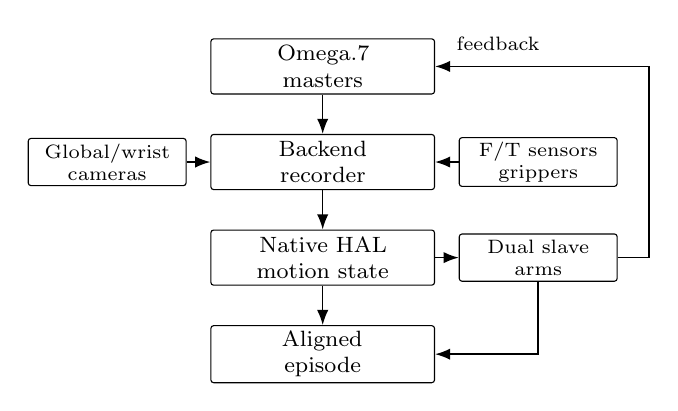
\begin{tikzpicture}[baseline=(current bounding box.north),
      node distance=5mm and 3mm,
      block/.style={draw, rounded corners=1pt, align=center, font=\footnotesize,
                    minimum height=7mm, text width=27mm, inner sep=2pt},
      smallblock/.style={draw, rounded corners=1pt, align=center, font=\scriptsize,
                    minimum height=6mm, text width=19mm, inner sep=1.5pt},
      arr/.style={-Latex, line width=0.55pt}
    ]
      \node[block] (master) {Omega.7\\masters};
      \node[block, below=of master] (recorder) {Backend\\recorder};
      \node[block, below=of recorder] (hal) {Native HAL\\motion state};
      \node[block, below=of hal] (episode) {Aligned\\episode};

      \node[smallblock, left=of recorder] (vision) {Global/wrist\\cameras};
      \node[smallblock, right=of recorder] (contact) {F/T sensors\\grippers};
      \node[smallblock, right=of hal] (stage) {Dual slave\\arms};

      \draw[arr] (master) -- (recorder);
      \draw[arr] (recorder) -- (hal);
      \draw[arr] (hal) -- (episode);
      \draw[arr] (vision) -- (recorder);
      \draw[arr] (contact) -- (recorder);
      \draw[arr] (hal) -- (stage);
      \draw[arr] (stage.south) |- (episode.east);
      \draw[arr] (stage.east) -- ++(4mm,0) |- (master.east);
      \node[font=\scriptsize, anchor=south west, xshift=1.5mm, yshift=0.8mm]
        at (master.east) {feedback};
    \end{tikzpicture}}
    \vspace{0.5mm}
    \parbox{0.95\linewidth}{\centering\small (b) English data-flow abstraction of the multimodal teleoperation stack.}
  \end{minipage}
  \caption{Overview of the proposed multimodal teleoperation data
  collection platform. The mechanical layout is a dual-arm micro-motion
  workstation, while the software pipeline converts heterogeneous sensor
  streams into aligned learning episodes.}
  \label{fig:overview}
\end{figure*}

\section{Related Work}
\textbf{Microassembly and micromanipulation.}
Microassembly technologies have long combined serial manipulation,
parallel organization, self-assembly, and task-specific fixtures.
Cohn et al.~\cite{cohn1998microassembly} describe why MEMS assembly
cannot be treated as a simple extension of macro-scale pick-and-place:
release, adhesion, and interconnection are fundamental challenges.
This motivates a platform that records force and pose, not only images.

\textbf{Haptic teleoperation at small scales.}
Bolopion and Regnier~\cite{bolopion2013haptic} review haptic feedback
teleoperation for micromanipulation and microassembly. Their discussion
is directly relevant to this system because the operator controls a
scaled remote tool and receives visual/force cues. The present paper
extends that idea toward dataset generation: the haptic loop is also a
source of expert demonstrations.

\textbf{Visual servoing and multi-view feedback.}
Visual servoing uses camera measurements inside a control loop
\cite{chaumette2006visual}. For microdevice assembly, camera feedback is
necessary but insufficient: contact may occur before large visual changes
are visible, and occlusion often appears near the final alignment stage.
Therefore, the proposed system records synchronized vision, stage state,
and force/torque signals.

\textbf{Robot learning from teleoperation.}
ALOHA demonstrates that low-cost bimanual teleoperation can collect
demonstrations for fine manipulation tasks~\cite{zhao2023aloha}. Open
X-Embodiment shows that standardized multi-robot datasets can support
generalist policies~\cite{oneill2024openx}. LeRobot further emphasizes
the importance of common dataset formats and reusable training tools
\cite{cadene2026lerobot}. These works motivate storing microassembly
episodes as synchronized videos and state/action tables.

\section{System Requirements}
The platform is designed for microdevice assembly tasks such as
alignment, insertion, light contact, and fragile part positioning. It
must satisfy four requirements.

\textbf{R1: Cross-scale motion mapping.}
Human input occurs at millimeter-to-centimeter scale, while the slave
stage must execute micrometer-level increments. The controller must
scale, filter, and limit this motion.

\textbf{R2: Multimodal observation.}
No single sensor is sufficient. Global vision shows workspace context;
wrist cameras provide local views; force/torque sensing detects contact;
encoders report actual stage motion; gripper telemetry reports grasp
state.

\textbf{R3: Causal alignment.}
The dataset must preserve temporal order. A frame should not pair an
image before contact with a force sample after contact. Alignment
quality must therefore be measured, not assumed.

\textbf{R4: Learning-ready episodes.}
The final output should be compatible with modern robot-learning
pipelines: video observations, numeric state/action arrays, metadata,
and per-frame quality labels.

\section{Hardware and Control Architecture}
The physical workstation is shown in Fig.~\ref{fig:overview}(a). It
uses two symmetric micro-motion slave arms. Each side can be described
as a serial chain of linear and rotary micro-stages ending in a force
sensor and gripper. The current engineering configuration uses three
cameras, two force/torque sensor channels, two Omega.7 haptic master
devices, and two parallel grippers.

\begin{table}[t]
  \centering
  \footnotesize
  \caption{Main hardware and data roles in the platform.}
  \label{tab:hardware}
  \begin{tabular}{@{}L{0.26\linewidth}L{0.28\linewidth}L{0.36\linewidth}@{}}
    \toprule
    Subsystem & Typical role & Recorded signal \\
    \midrule
    Linear stages & $x,y,z$ motion & position, pulses \\
    Rotary stages & roll/pitch/yaw & angle, pulses \\
    Omega.7 masters & operator intent & pose, buttons, gap \\
    Global camera & workspace view & RGB stream \\
    Wrist cameras & local views & RGB streams \\
    F/T sensors & contact feedback & force, torque \\
    Parallel grippers & grasp/release & opening, target \\
    \bottomrule
  \end{tabular}
\end{table}

The software stack separates real-time device access from dataset
assembly. A native hardware abstraction layer (HAL) communicates with
motion hardware and haptic devices. A backend service configures the
system, receives telemetry, starts recording sessions, and assembles
episodes. This separation avoids placing camera capture, force sampling,
UI state, motion-card calls, and dataset writing inside one monolithic
process.

\subsection{Calibration and safety constraints}
For a microassembly workstation, calibration is part of the data
definition rather than a separate maintenance activity. The same command
vector can mean different physical motion if the axis order, direction
signs, pulse-per-unit coefficients, camera mounting, or tool offsets are
changed. Therefore, each recorded session should store a compact
calibration snapshot: master-to-slave scale factors, linear-stage
conversion coefficients, rotary-stage conversion coefficients, gripper
open/close ranges, camera identifiers, image resolution, and the active
workspace limits. These values allow a later user to interpret the
episode as a physical trace instead of a collection of unrelated sensor
messages.

The workstation uses a master-slave control loop, so safety constraints
must be enforced before a command is sent to the motion layer. The first
constraint is geometric: each linear and rotary stage is bounded by a
soft limit derived from the mechanical travel range and the current task
fixture. The second constraint is dynamic: master-hand increments are
filtered through dead zones, gain scaling, and velocity limits so that
operator tremor does not become a destructive micro-motion command. The
third constraint is contact-aware: force and torque values are monitored
as both feedback and data-quality signals. When contact exceeds a
warning threshold, the frame should be labeled; when it exceeds a stop
threshold, command output should be suppressed until the operator
re-enters a safe state.

This calibration-and-safety design also makes the dataset more useful
for learning. A policy trained from demonstrations should know whether
an action came from normal teleoperation, a saturated soft limit, or an
operator recovery. Without these labels, a model may imitate clipped
commands or contact-recovery motions as if they were ordinary assembly
behavior. In the proposed schema, safety events are therefore written
beside the state/action frame instead of being treated as private runtime
logs.

\section{Kinematic Mapping}
The micro-motion platform can be modeled as a serial chain with
translation and rotation stages. Fig.~\ref{fig:kinematics} shows the
frame assignment used to reason about the end-effector pose. Although
the implementation does not need to solve a symbolic model at every
control cycle, the model is useful for explaining axis order, signed
pulse-per-unit coefficients, and the relation between low-level stage
motion and end-effector pose.

\begin{figure}[t]
  \centering
  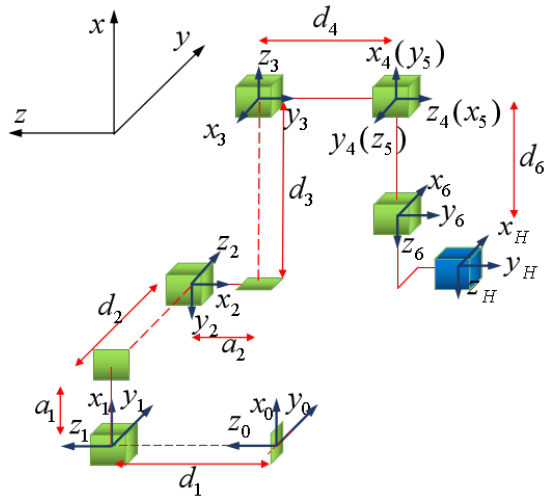
\includegraphics[width=0.88\linewidth]{figures/paper_kinematic_frames.png}
  \caption{Kinematic frame assignment for the six-degree-of-freedom
  micro-motion platform. The notation is used to relate stage variables
  to the end-effector pose.}
  \label{fig:kinematics}
\end{figure}

For adjacent frames, the homogeneous transform is written as
\begin{equation}
{}^{i-1}_{i}T =
\begin{bmatrix}
c_i & -s_i & 0 & a_{i-1}\\
s_ic_{\alpha} & c_ic_{\alpha} & -s_{\alpha} & -s_{\alpha}d_i\\
s_is_{\alpha} & c_is_{\alpha} & c_{\alpha} & c_{\alpha}d_i\\
0 & 0 & 0 & 1
\end{bmatrix},
\end{equation}
where $c_i=\cos\theta_i$, $s_i=\sin\theta_i$,
$c_{\alpha}=\cos\alpha_{i-1}$, and
$s_{\alpha}=\sin\alpha_{i-1}$. The end-effector pose is
\begin{align}
{}^{0}_{H}T &= A_1A_2A_3A_4A_5A_6,\\
{}^{0}_{H}T &=
\begin{bmatrix}
\mathbf{n} & \mathbf{o} & \mathbf{a} & \mathbf{p}\\
0 & 0 & 0 & 1
\end{bmatrix}.
\end{align}

\begin{table}[t]
  \centering
  \small
  \caption{D-H-style parameters used for the micro-motion chain.}
  \label{tab:dh}
  \begin{tabular}{@{}ccccc@{}}
    \toprule
    $i$ & $\alpha_{i-1}$ & $a_{i-1}$ & $d_i$ & $\theta_i$ \\
    \midrule
    1 & $0$ & $0$ & $d_1$ & $0$ \\
    2 & $-90^\circ$ & $a_1$ & $d_2$ & $90^\circ$ \\
    3 & $90^\circ$ & $a_2$ & $d_3$ & $-90^\circ$ \\
    4 & $-90^\circ$ & $0$ & $d_4$ & $\theta_4-90^\circ$ \\
    5 & $-90^\circ$ & $0$ & $0$ & $\theta_5-90^\circ$ \\
    6 & $90^\circ$ & $0$ & $d_6$ & $\theta_6-90^\circ$ \\
    $H$ & $0$ & $0$ & $d_H$ & $0$ \\
    \bottomrule
  \end{tabular}
\end{table}

In the controller, this model becomes a practical mapping from master
increments to stage commands. Translation is represented in micrometers,
rotation in degrees, and each axis is converted to signed pulses before
being sent to the motion layer. Dead zones, per-axis gains, velocity
limits, and soft limits are applied before the command reaches the
hardware. These filters are not cosmetic; they are required because
microassembly is sensitive to tremor, over-travel, and contact-induced
damage.

\section{Multimodal Recording and Alignment}
The recorder operates around a target learning frame rate, while
individual devices update at different rates. Cameras are relatively
slow, haptic-state and gripper streams are faster, and motion hardware
can update faster still. The system therefore stores each stream in a
source-specific ring buffer and assembles a training frame only after a
small alignment delay.

\subsection{Data schema}
Each episode contains synchronized camera streams and numeric tables.
The vision part stores a global view and two wrist views. The state part
stores left/right stage state, gripper opening, force/torque values, and
optional raw pulse positions. The action part stores the master-hand
increment or target command issued at that time. A separate quality
report records skew, timeout, stale samples, and cache usage.

\begin{table}[t]
  \centering
  \footnotesize
  \caption{Episode fields and their intended use.}
  \label{tab:episode}
  \begin{tabular}{@{}L{0.30\linewidth}L{0.58\linewidth}@{}}
    \toprule
    Field group & Examples \\
    \midrule
    Images & global view, left/right wrist views \\
    State & stage pose, pulses, gripper opening, force/torque \\
    Actions & master increment, side, gripper target, speed mode \\
    Metadata & calibration, axis maps, limits, FPS \\
    Quality & skew, timeout, stale source, dropped source \\
    \bottomrule
  \end{tabular}
\end{table}

\subsection{Timestamp alignment}
Let $t_k$ be the nominal timestamp of the $k$-th training frame. For
each source $s$, the recorder chooses the nearest available sample
\begin{equation}
x_s^\star(k) = \arg\min_{x_s \in \mathcal{B}_s}
\left| \tau(x_s) - (t_k-\Delta) \right|,
\end{equation}
where $\mathcal{B}_s$ is the source buffer, $\tau(x_s)$ is the monotonic
timestamp, and $\Delta$ is a fixed alignment delay. The sample is accepted
if
\begin{equation}
\left| \tau(x_s^\star) - (t_k-\Delta) \right| < \epsilon_s,
\end{equation}
where $\epsilon_s$ is a source-dependent skew threshold. If the threshold
is exceeded, the frame may still be written, but it is marked in the
quality report. This is preferable to silently discarding an expensive
expert demonstration or silently writing a misleading frame.

\subsection{Quality control for demonstrations}
A microassembly demonstration is usually expensive: it requires a
prepared fixture, a stable optical view, a trained operator, and fragile
components. For this reason, the recorder should preserve imperfect
episodes while making their imperfections explicit. The proposed quality
report uses frame-level flags rather than a single pass/fail decision.
For example, a frame can be marked as camera-stale but force-valid, or
as force-delayed but visually correct. Downstream training code can then
discard, down-weight, or separately analyze these cases.

Four quality dimensions are especially important. The first is temporal
skew, which measures the difference between each source timestamp and
the target learning timestamp. The second is source availability, which
records whether a modality was missing, repeated from cache, or sampled
from a stale buffer. The third is physical consistency, which checks
whether state changes agree with commanded directions and soft-limit
status. The fourth is task validity, which records whether the operator
was executing the intended phase, recovering from an error, or resetting
the fixture. The final dimension is partly semantic, but it matters for
learning because recovery behavior should not be mixed blindly with
nominal assembly behavior.

\begin{table}[t]
  \centering
  \footnotesize
  \caption{Frame-level quality labels written with each episode.}
  \label{tab:quality}
  \begin{tabular}{@{}L{0.28\linewidth}L{0.58\linewidth}@{}}
    \toprule
    Label & Meaning \\
    \midrule
    {\scriptsize skew\_ms} & largest source-to-frame time error \\
    {\scriptsize stale\_source} & reused sample from cache \\
    {\scriptsize drop\_source} & missing modality at frame time \\
    {\scriptsize limit\_active} & command clipped by limits \\
    {\scriptsize contact\_warn} & force/torque warning \\
    {\scriptsize phase} & approach/align/grasp/transfer/release/reset \\
    \bottomrule
  \end{tabular}
\end{table}

The same labels support rapid debugging during experiments. If a policy
fails in a later replay test, the researcher can inspect whether the
demonstrations contained high camera skew, repeated force samples, or a
large number of limit-active frames. This turns the data pipeline into a
diagnostic tool rather than a passive file writer.

\begin{table}[t]
  \centering
  \footnotesize
  \caption{Representative timing targets used by the recorder.}
  \label{tab:timing}
  \begin{tabular}{@{}L{0.34\linewidth}L{0.22\linewidth}L{0.34\linewidth}@{}}
    \toprule
    Item & Value & Purpose \\
    \midrule
    Learning FPS & 30 Hz & dataset time base \\
    Haptic state & 100 Hz & pose and grip gap \\
    Motion state & up to 1000 Hz & encoder/pulse state \\
    Alignment delay & 100 ms & async wait \\
    Buffer retention & 3 s & nearest lookup \\
    Camera skew & 35 ms & image flag \\
    Force skew & 10 ms & contact flag \\
    \bottomrule
  \end{tabular}
\end{table}

\section{Evaluation Scenarios}
The platform should be evaluated with tasks that expose different
failure modes of microdevice assembly. A single pick-and-place example
is not sufficient, because it may test only visual alignment while
leaving force timing, gripper coordination, and recovery behavior
unmeasured. The following scenarios are therefore proposed as a compact
benchmark suite for the workstation.

\textbf{Free-space positioning.} The operator moves one slave arm through
a sequence of commanded poses without intentional contact. This scenario
tests axis signs, scale factors, soft limits, and the basic mapping from
Omega.7 motion to micro-stage increments. The expected data signature is
smooth master motion, low force magnitude, and monotonic stage response
under the chosen coordinate convention.

\textbf{Visual alignment.} A microcomponent or target mark is placed in
the global view and then refined in the wrist view. The operator aligns
the tool tip with the target while keeping contact force near zero. This
scenario tests whether global and local cameras are synchronized with
stage state. It is also useful for measuring whether the dataset records
the hand motion that caused each visible change, rather than pairing an
image with a future or past command.

\textbf{Light-contact approach.} The slave tool approaches a surface
until a small force threshold is reached, then retreats or slides along
the surface. This scenario is important because many microassembly
errors occur before the camera view changes dramatically. A correct
recording should show the force rise at the same logical step as the
approach command and the encoder change. If the force peak appears one
or two frames away from the action that caused it, the dataset is not
ready for contact-sensitive learning.

\textbf{Bimanual handoff.} The left and right slave arms coordinate a
small part transfer. One side stabilizes the part while the other side
grasps, releases, or reorients it. This scenario tests cross-arm
synchronization, gripper-state recording, and the ability to represent
two action streams in one learning frame. It also exposes whether the
quality report can distinguish a normal handoff from a recovery after a
failed grasp.

\begin{table}[t]
  \centering
  \footnotesize
  \caption{Suggested task-level checks for the platform.}
  \label{tab:scenarios}
  \begin{tabular}{@{}L{0.30\linewidth}L{0.55\linewidth}@{}}
    \toprule
    Scenario & Main checks \\
    \midrule
    Free-space motion & axis signs, gains, soft limits \\
    Visual alignment & camera-state skew, view consistency \\
    Light contact & force timing, contact labels \\
    Bimanual handoff & cross-arm sync, gripper state \\
    \bottomrule
  \end{tabular}
\end{table}

For each scenario, the system should report both human-readable plots and
machine-readable quality statistics. Useful plots include image-frame
timelines, force magnitude over time, stage displacement over time, and
skew histograms for each source. Useful statistics include missing-frame
rate, maximum skew, median skew, number of limit-active frames, number of
contact-warning frames, and the distribution of task phases. These
metrics do not prove that a future learned policy will succeed, but they
prevent a common failure case: collecting many visually plausible
episodes that are temporally inconsistent or physically ambiguous.

\balance
\section{Validation Plan}
The system should be evaluated before collecting large demonstrations.
The minimal validation loop is:
\begin{enumerate}[leftmargin=1.3em,itemsep=1pt,topsep=2pt]
  \item Start the HAL and backend services and verify that motion
  hardware, haptic masters, cameras, force sensors, and grippers are
  online.
  \item Move each Omega.7 master and verify that the mapped slave arm
  responds in the intended direction under soft limits.
  \item Open and close each haptic gripper input and verify that the
  corresponding physical gripper follows without blocking the other side.
  \item Record a short episode and check that all camera, state, force,
  gripper, and action fields are present.
  \item Inspect skew histograms and source-drop labels before using the
  episode for policy learning.
\end{enumerate}

Success should be measured at three levels. At the hardware level, the
platform should respect motion limits and avoid contact overload. At the
data level, the episode should have low missing-rate and bounded skew. At
the learning level, demonstrations should support policies that reproduce
alignment and contact behaviors without requiring hidden manual
intervention.

\section{Discussion}
The proposed system differs from large macro-scale robot datasets in
three ways. First, the task is contact-sensitive at a much smaller scale,
so force and pulse-state logging are as important as images. Second, the
mechanical layout is based on micro-motion stages rather than common
industrial arms, which makes axis calibration and signed pulse mapping
part of the dataset contract. Third, the user interface is a haptic
master-slave loop, so the master-hand state is both a control input and a
learning signal.

The design also has limitations. Cameras at 30 Hz cannot fully capture
fast contact transients. Force sensing and encoder state help, but
high-speed events may still require additional instrumentation. The
mapping gains and dead zones are currently engineering parameters; future
work should adapt them online based on operator intent, force cues, and
task phase. Finally, a dataset format alone does not guarantee useful
learning. The quality report must be connected to policy training so that
badly aligned frames can be filtered or down-weighted.

\section{Conclusion}
This paper described an English CVPR-style design for multimodal
teleoperation data collection in microdevice assembly. The system uses a
dual-arm micro-motion workstation, haptic master devices, cameras,
force/torque sensing, grippers, and a backend recorder to produce aligned
learning episodes. Public work in microassembly, haptic teleoperation,
visual servoing, bimanual imitation learning, and robot dataset tooling
motivates the design. The central lesson is that microassembly data must
be treated as a synchronized physical record, not merely as a video log:
each frame should connect observation, action, state, and contact.

\begin{thebibliography}{9}
\bibitem{cohn1998microassembly}
M.~B. Cohn, K.~F. Bohringer, J.~M. Noworolski, A.~Singh, C.~G. Keller,
K.~Y. Goldberg, and R.~T. Howe.
\newblock Microassembly technologies for MEMS.
\newblock In \emph{Proc. SPIE}, 3512, 1998.
\newblock doi:10.1117/12.324061.

\bibitem{bolopion2013haptic}
A.~Bolopion and S.~Regnier.
\newblock A review of haptic feedback teleoperation systems for
micromanipulation and microassembly.
\newblock \emph{IEEE Transactions on Automation Science and Engineering},
10(3):496--502, 2013.
\newblock doi:10.1109/TASE.2013.2245122.

\bibitem{chaumette2006visual}
F.~Chaumette and S.~Hutchinson.
\newblock Visual servo control, Part I: Basic approaches.
\newblock \emph{IEEE Robotics \& Automation Magazine}, 13(4):82--90, 2006.
\newblock doi:10.1109/MRA.2006.250573.

\bibitem{zhao2023aloha}
T.~Z. Zhao, V.~Kumar, S.~Levine, and C.~Finn.
\newblock Learning fine-grained bimanual manipulation with low-cost hardware.
\newblock In \emph{Robotics: Science and Systems}, 2023.

\bibitem{chi2023diffusion}
C.~Chi, Z.~Xu, S.~Feng, E.~Cousineau, Y.~Du, B.~Burchfiel, R.~Tedrake,
and S.~Song.
\newblock Diffusion Policy: Visuomotor policy learning via action diffusion.
\newblock In \emph{Robotics: Science and Systems}, 2023.

\bibitem{oneill2024openx}
Open X-Embodiment Collaboration, A.~O'Neill, A.~Rehman, A.~Gupta, et al.
\newblock Open X-Embodiment: Robotic learning datasets and RT-X models.
\newblock In \emph{IEEE International Conference on Robotics and Automation},
2024.
\newblock doi:10.1109/ICRA57147.2024.10611477.

\bibitem{cadene2026lerobot}
R.~Cadene, S.~Aliberts, F.~Capuano, M.~Aractingi, A.~Zouitine,
P.~Kooijmans, J.~Choghari, M.~Russi, C.~Pascal, S.~Palma, M.~Shukor,
J.~Moss, A.~Soare, D.~Aubakirova, Q.~Lhoest, Q.~Gallouedec, and T.~Wolf.
\newblock LeRobot: An open-source library for end-to-end robot learning.
\newblock arXiv:2602.22818, 2026.
\end{thebibliography}

\end{document}
